\documentclass{article}
\usepackage[utf8]{inputenc}
\usepackage[parfill]{parskip}

\usepackage[a4paper,
margin=0.6in,top=1.2in,
bottom=1.5in]{geometry}
\usepackage{fancyhdr}
\pagestyle{fancy}
\fancyhf{}
\rhead{CS695 Assignment 4}
\lhead{200050157-20d070006}
\cfoot{Page \thepage}
\renewcommand{\footrulewidth}{0.4pt}

\usepackage{algorithm2e}
\usepackage{comment}
\usepackage{amsmath} 
\usepackage{amsthm}
\usepackage{amssymb} 
\usepackage{mathtools}
\usepackage{esint}
\newtheorem{result}{Result}
\newtheorem{theorem}{Theorem}

\usepackage{graphicx} 
\usepackage{floatrow} 
\usepackage{listings} 
\usepackage{url}
\usepackage{xcolor}
\usepackage[font={it}]{caption}
\usepackage{pgffor}
\usepackage{hyperref}

% https://tex.stackexchange.com/questions/654207/help-with-looping-through-a-folder-to-insert-all-images-within
\newcommand*{\VsIntervalImageNames}
{
average_cpu_usage-vs-interval_numbers.png,
% full_scans-vs-interval_numbers.png,
general_profit-vs-interval_numbers.png,
pages_shared-vs-interval_numbers.png,
pages_sharing-vs-interval_numbers.png,
pages_unshared-vs-interval_numbers.png,
pages_volatile-vs-interval_numbers.png
}

\newcommand*{\VsIntervalImageNamesNoWorkload}
{
average_cpu_usage-vs-interval_numbers.png,
% full_scans-vs-interval_numbers.png,
general_profit-vs-interval_numbers.png,
pages_shared-vs-interval_numbers.png,
pages_sharing-vs-interval_numbers.png
% pages_unshared-vs-interval_numbers.png,
% pages_volatile-vs-interval_numbers.png
}

\newcommand*{\VsIntervalImageNamesWorkload}
{
average_cpu_usage-vs-interval_numbers.png,
% full_scans-vs-interval_numbers.png,
general_profit-vs-interval_numbers.png,
pages_shared-vs-interval_numbers.png,
pages_sharing-vs-interval_numbers.png,
% pages_unshared-vs-interval_numbers.png,
pages_volatile-vs-interval_numbers.png
}

\newcommand*{\VsIntervalImageNamesOld}
{
cpu_usage_vs_interval.png,
general_profit_vs_interval.png,
pages_shared_vs_interval.png,
pages_sharing_vs_interval.png
}

\newcommand*{\VsIntervalImageNamesProc}
{
proc-ksm_merging_pages-vs-interval_numbers.png,
proc-ksm_process_profit-vs-interval_numbers.png,
proc-ksm_rmap_items-vs-interval_numbers.png
}

\newcommand*{\ManualProgramsImageNames}
{
general_profit-vs-interval_numbers.png,
pages_shared-vs-interval_numbers.png,
pages_sharing-vs-interval_numbers.png,
pages_unshared-vs-interval_numbers.png
}

\newcommand*{\VsVmsImageNames}
{
average_cpu_usage-vs-vms.png,
% full_scans-vs-vms.png,
general_profit-vs-vms.png,
pages_shared-vs-vms.png,
pages_sharing-vs-vms.png,
pages_unshared-vs-vms.png,
pages_volatile-vs-vms.png
}

\newcommand*{\VsVmsImageNamesOld}
{
cpu_usage_vs_vm.png,
general_profit_vs_vm.png,
pages_shared_vs_vm.png,
pages_sharing_vs_vm.png
}

\newcommand*{\VsVmsImageNamesNoWorkload}
{
average_cpu_usage-vs-vms.png,
% full_scans-vs-vms.png,
general_profit-vs-vms.png,
pages_shared-vs-vms.png,
pages_sharing-vs-vms.png
% pages_unshared-vs-vms.png,
% pages_volatile-vs-vms.png
}

\newcommand*{\VsVmsImageNamesWorkload}
{
average_cpu_usage-vs-vms.png,
% full_scans-vs-vms.png,
general_profit-vs-vms.png,
pages_shared-vs-vms.png,
pages_sharing-vs-vms.png
% pages_unshared-vs-vms.png,
% pages_volatile-vs-vms.png
}

\newcommand*{\VsVmsImageNamesMemmgmt}
{
memory-vs-vms.png,
percent-vs-vms.png
}

\title{CS695 Assignment 4 Report}
\author{Virendra Kabra and Advaid Deepak \\ 200050157 - 20d070006}
\date{Spring 2024}

\begin{document}

\maketitle
\tableofcontents
\newpage

\section{Overview}

\subsection{KSM}

KSM (Kernel Samepage Merging) \cite{ksm_doc} is a memory-deduplication feature in Linux kernels. A common use-case for this is when we want to fit multiple VMs onto a single physical machine. For example, these VMs might be running the same OS or the same applications, and such data can be shared across them. KSM enables this by merging copies of the same page.

\subsection{Kernel Implementation of KSM}

We work with Linux Kernel v6.5 available with Ubuntu 22.04 LTS. A brief description of the KSM implementation \cite{ksm_impl} follows:

\begin{enumerate}
\item Data-structures
    \begin{itemize}
        \item Two red-black trees are used for storing pages: a stable tree and an unstable tree. Tree nodes are ordered by page contents.
        \item The stable tree holds pointers to all the merged pages (ksm pages). Each such page is write-protected. Two types of nodes are used: regular nodes that keep reverse mapping structures in a list, and chain nodes that hold lists of duplicate pages.
        \item The unstable tree holds pointers to pages which have been found to be unchanged for a certain period of time. These pages are not write-protected, hence the term ``unstable". This is similar to the hint entries from \texttt{[memmgmt]} paper \cite{memmgmt}.
    \end{itemize}
\item Workflow
    \begin{itemize}
        \item \texttt{ksm\_do\_scan}: The KSM daemon \texttt{ksmd} scans through all mergeable pages (e.g. \texttt{madvise}'d \texttt{MADV\_MERGEABLE} and anonymous) in each iteration.
        \item \texttt{cmp\_and\_merge\_page}: The hash value (checksum) of this page is computed. If checksum is same as seen in the previous iteration, it is inserted into the unstable tree or merged with another page from unstable tree into the stable one.
        \item This is different from the approach in \texttt{[memmgmt]} \cite{memmgmt} where hash value of a page is compared with hashes of other pages. Here, if the page hash is constant across full-scans, its entire content is compared against pages from tree pages using \texttt{memcmp} \cite{memcmp_pages}.
    \end{itemize}
\end{enumerate}

\newpage

\section{Parameters and Metrics}
\label{sec:params_metrics}

\subsection{Parameters}
\label{sec:params}

Our main script \texttt{orchestrate.sh} allows several command-line arguments, including the below parameters.

\begin{itemize}
    \item Number of VMs. Each VM runs Debian12 with 512MB memory and 4GB disk. We setup the first VM manually and clone the rest using \texttt{virsh}.
    \item Scan-rate: Scanning rate of mergeable pages by the KSM daemon. This can be varied with \texttt{pages\_to\_scan} - the number of pages to scan before \texttt{ksmd} sleeps, and with \texttt{sleep\_millisecs} - the daemon's sleep-time. Since both inversely affect the scan-rate, we list experiments with \texttt{pages\_to\_scan}.
    \item VM Workload: This is the workload that each VM runs. We experiment with no workload, and with variations of \texttt{stress-ng} \cite{stress_ng}. For \texttt{stress-ng}, we disable swapping and start 2 workers per VM continuously calling mmap/munmap and writing to the allocated memory, varying advise \texttt{mergeable} and \texttt{unmergeable}. Other options are also used, and are discussed with VM experiments \ref{exp_vms}.
    \item For experiments without VMs, a different set of parameters is varied. Details below in \ref{exp_no_vm}.
\end{itemize}

\subsection{Metrics}
\label{sec:metrics}

All monitoring happens via the \texttt{monitor\_ksm.sh} script. This is invoked from the main orchestrator script. We note that the monitoring is not CPU-intensive, as can be observed in the experiments. Average CPU usage remains almost the same even as we increase the monitoring frequency by 60 times (per-minute to per-second granularity). Some metrics of interest are listed below.

\begin{itemize}
    \item CPU usage: Average CPU usage on the machine in the interval.%This is not just for KSM daemon as we also want to see effect of VMs.
    \item \texttt{pages\_shared}: Number of shared pages being used, i.e., count of distinct KSM pages. Same as number of regular nodes in the stable tree.
    \item \texttt{pages\_sharing}: Number of duplicate pages reclaimed. This is disjoint from pages counted in \texttt{pages\_shared}.
    \item \texttt{pages\_unshared}: Number of nodes in the unstable tree, i.e., pages that haven't changed since last full-scan but are yet to be shared.
    \item General Profit: Overall measure of how effective KSM is. Computed as \newline\texttt{pages\_sharing * PAGE\_SIZE - rmap\_items * sizeof(rmap\_item)}
\end{itemize}

These are plotted both against intervals and number of VMs.

When plotting against number of VMs, we take values from the last interval. This captures stabilized metrics.

In some cases, we also refer to per-process KSM stats. These are obtained from \texttt{/proc/<pid>/ksm\_stats}.

\section{File-Structure and Usage Instructions}

Please refer to the project README for a description of files, along with detailed setup and usage instructions.

\newpage

\section{Experiments without VMs}
\label{exp_no_vm}

These experiments are performed to understand the internal working of KSM.

In these experiments, we allocate two KSM-mergeable arrays and observe effects on the metrics. Steps: allocate \texttt{array1} and \texttt{array2} in 10-second intervals. \texttt{array[i]=i} for both arrays. 10-seconds after both arrays have been allocated, some part of \texttt{array1} is modified to see KSM working and effect on metrics.

% 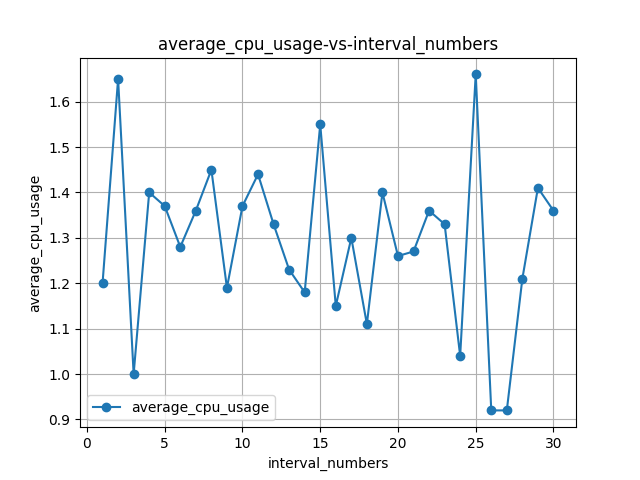
\includegraphics[width=0.3\textwidth]{Images/manual_programs/modifyBy_h/average_cpu_usage-vs-interval_numbers.png}\hspace{0pt}

Below, for all three experiments, we observe that \texttt{general\_profit} is negative for initial intervals. This happens because no sharing has been done yet but rmap items are being created and unstable tree is being populated.

\begin{enumerate}

\item After sharing stabilizes, exactly one page is modified and hence unmerged. This is clearly seen in the logs.

\begingroup
\raggedright%
\foreach \x in \ManualProgramsImageNames
{
\includegraphics[width=0.2\textwidth]{Images/manual_programs/modifyBy_s/\x}\hspace{0pt}
}
\captionof{figure}{Changing \texttt{array1[0]} to $-1$}
\endgroup

\item A dip in the middle happens due to unmerging of first half of arrays. But after that, half the pages of \texttt{array1} themselves can be merged as all values are $-1$, increasing the profit and shared pages.

\begingroup
\raggedright%
\foreach \x in \ManualProgramsImageNames
{
\includegraphics[width=0.2\textwidth]{Images/manual_programs/modifyBy_h/\x}\hspace{0pt}
}
\captionof{figure}{Changing half of first array to all $-1$s}
\endgroup

\item Similar to previous experiment, a dip is seen in the middle. But now since modified values are distinct, they cannot be merged. Since the values are not changing after that, a smaller peak is visible at the end in \texttt{pages\_unshared}.

\begingroup
\raggedright%
\foreach \x in \ManualProgramsImageNames
{
\includegraphics[width=0.2\textwidth]{Images/manual_programs/modifyBy_m/\x}\hspace{0pt}
}
\captionof{figure}{Changing half of first array by \texttt{array1[i]=-i}}
\endgroup

\end{enumerate}

\newpage

\section{Experiments with VMs}
\label{exp_vms}

We performed experiments by varying the parameters discussed in \ref{sec:params}. For each experiment, we monitored the metrics described in \ref{sec:metrics}.

An important thing to note is that recorded metrics are for \textbf{system-wide} deduplication, as \texttt{ksmd} is running on the host machine. Hence, some noise is expected from merging and unsharing of other processes' pages.

\subsection{Experiment 1}
\label{exp_vms:1}

In this experiment, the scan rate is 1000 pages per 20 milliseconds. No workload was put on the VMs. We monitor for 30 intervals each lasting 60 sec.

\subsubsection{Metric vs Interval}

\begingroup
\raggedright%
\foreach \x in \VsIntervalImageNamesNoWorkload
{
\includegraphics[width=0.2\textwidth]{Images/logs_2024_04_19_14_26/plots/3/\x}\hspace{0pt}
}
\captionof{figure}{}
\endgroup

Three VMs were ran for the above plots, without workloads. We observe random variation in CPU usage. General profit and \texttt{pages\_sharing} \textit{slightly} decrease after an initial large value. This may be attributed to VMs writing to common pages after an initial phase. This may be due to noise as well - we do not observe this trend when experiments in the same setup with a larger number of VMs (\ref{exp_vms:8}). The slight increment in \texttt{pages\_shared} around 15 minutes may either be because of noise or because of sharing in 2 of the 3 VMs.

\begingroup
\raggedright%
\foreach \x in \VsIntervalImageNamesProc
{
\includegraphics[width=0.2\textwidth]{Images/logs_2024_04_19_14_26/plots/3/\x}\hspace{0pt}
}
\captionof{figure}{}
\endgroup

Each line in the above plots is for a VM process. \texttt{ksm\_merging\_pages} is the sum of \texttt{pages\_sharing} and \texttt{pages\_shared} \cite{ksm_merging_pages_impl}. It is higher for the first VM as it is more likely that de-duplication of later VMs happens \textit{due to} memory regions of the first one. Further, we observe an increase in sharing for VMs 2 and 3 in the middle. Again, note that the differences are very small. We do not observe these in a later experiment \ref{exp_vms:8}.

\subsubsection{Metric vs VM}
\begingroup
\raggedright%
\foreach \x in \VsVmsImageNamesNoWorkload
{
\includegraphics[width=0.2\textwidth]{Images/logs_2024_04_19_14_26/plots/vms/\x}\hspace{0pt}
}
\captionof{figure}{}
\endgroup

We observe that all KSM metrics increase with increase in number of VMs. This is expected because as number of VMs increase, there is that much more opportunity for page-sharing. This observation is common for all experiments.

\subsection{Experiment 2}
\label{exp_vms:2}

This experiment is similar to \ref{exp_vms:1}, with the only variation being in the scan rate: we increased it to $10000$ pages per $20$ milliseconds.

\subsubsection{Metric vs Interval}

\begingroup
\raggedright%
\foreach \x in \VsIntervalImageNamesOld
{
\includegraphics[width=0.2\textwidth]{Images/logs_2024_04_16_19_06/plots/3/\x}\hspace{0pt}
}
\captionof{figure}{}
\endgroup

We observe that, owing to the increased scan rate, sharing happens quicker compared to the previous experiment. Also, an increased CPU usage is observed. This may be attributed to the KSM daemon. However, the profit and sharing values are almost same as before. This is because the earlier scan-rate is sufficiently large to scan through mergeable pages.

\subsubsection{Metric vs VM}
\begingroup
\raggedright%
\foreach \x in \VsVmsImageNamesOld
{
\includegraphics[width=0.2\textwidth]{Images/logs_2024_04_16_19_06/plots/vms/\x}\hspace{0pt}
}
\captionof{figure}{}
\endgroup

Similar observations as in the previous experiment follow.

\subsection{Experiment 3}
\label{exp_vms:3}

This experiment is similar to \ref{exp_vms:1} (scan-rate: 1000 pages per 20 ms) except there is a workload in the VMs. This workload is created using stress-ng. Details of this workload were discussed above in \ref{sec:params}. Swapping is disabled in the VMs. We run stress-ng for only the first half of the experiment to contrast metrics with/without workloads. Further, the advise for stress-ng is \texttt{unmergeable}.

\subsubsection{Metric vs Interval}

\begingroup
\raggedright%
\foreach \x in \VsIntervalImageNamesWorkload
{
\includegraphics[width=0.2\textwidth]{Images/logs_2024_04_18_18_04/plots/3/\x}\hspace{0pt}
}
\captionof{figure}{}
\endgroup

Since we run stress-ng for only first half of the experiment, the CPU usage is higher in the first half. Sharing happens more in the second half when stress-ng is turned off as it repeatedly mmaps/unmaps and writes to certain pages reducing the number of pages which can be shared. Trend in volatile pages is characteristic of the workload. This pattern is common to all subsequent experiments where this workload is used.

\subsubsection{Metric vs VM}
\begingroup
\raggedright%
\foreach \x in \VsVmsImageNamesWorkload
{
\includegraphics[width=0.2\textwidth]{Images/logs_2024_04_18_18_04/plots/vms/\x}\hspace{0pt}
}
\captionof{figure}{}
\endgroup

\subsection{Experiment 4}
\label{exp_vms:4}

This experiment is similar to \ref{exp_vms:3} except we scan 10000 pages in each 20 ms interval.

\subsubsection{Metric vs Interval}

\begingroup
\raggedright%
\foreach \x in \VsIntervalImageNamesWorkload
{
\includegraphics[width=0.2\textwidth]{Images/logs_2024_04_18_18_37/plots/3/\x}\hspace{0pt}
}
\captionof{figure}{}
\endgroup

\subsubsection{Metric vs VM}
\begingroup
\raggedright%
\foreach \x in \VsVmsImageNamesWorkload
{
\includegraphics[width=0.2\textwidth]{Images/logs_2024_04_18_18_37/plots/vms/\x}\hspace{0pt}
}
\captionof{figure}{}
\endgroup

Similar observations follow as in \ref{exp_vms:3}. Higher CPU usage may be attributed to the increased scan rate.

\subsection{Experiment 5}
\label{exp_vms:5}

This experiment is similar to \ref{exp_vms:3} (scan-rate: 1000 pages per 20 ms) except that the advise for stress-ng is \texttt{mergeable}. This was \texttt{unmergeable} in \ref{exp_vms:3}.

\subsubsection{Metric vs Interval}
\begingroup
\raggedright%
\foreach \x in \VsIntervalImageNamesWorkload
{
\includegraphics[width=0.2\textwidth]{Images/logs_2024_04_20_07_37/plots/3/\x}\hspace{0pt}
}
\captionof{figure}{}
\endgroup

We observe that the sharing does not improve even though the workload advise was \texttt{mergeable}. The number of volatile pages too is same as seen in the last two experiments. This is due to the workload nature: it repeatedly mmaps/unmaps pages with 0 wait. So we expect no significant deviations from the experiments where advise was \texttt{unmergeable}.

\subsubsection{Metric vs VM}

\begingroup
\raggedright%
\foreach \x in \VsVmsImageNamesWorkload
{
\includegraphics[width=0.2\textwidth]{Images/logs_2024_04_20_07_37/plots/vms/\x}\hspace{0pt}
}
\captionof{figure}{}
\endgroup

\begingroup
\raggedright%
\foreach \x in \VsVmsImageNamesMemmgmt
{
\includegraphics[width=0.4\textwidth]{Images/logs_2024_04_20_07_37/plots/vms/\x}\hspace{0pt}
}
\captionof{figure}{}
\endgroup

The pattern observed is similar to that in \texttt{memmgmt} \cite{memmgmt}, where VM memory, shared memory, and reclaimed memory increase as the number of VMs increase. The sharing percentage tends to flatten after 2 VMs, as seen clearly in \ref{exp_vms:8}.

\subsection{Experiment 6}
\label{exp_vms:6}

This experiment is similar to \ref{exp_vms:5}. Since we could not get the benefits of advising \texttt{mergeable}, we now also waited for $10$ seconds before unmapping the mmap'ed memory regions. This was by adding \texttt{--vm-hang 10} in the VM workload.

\subsubsection{Metric vs Interval}

\begingroup
\raggedright%
\foreach \x in \VsIntervalImageNamesWorkload
{
\includegraphics[width=0.2\textwidth]{Images/logs_2024_04_26_22_27/plots/3/\x}\hspace{0pt}
}
\captionof{figure}{}
\endgroup

We observe an increase in the profit and shared pages in the first half (that is, when the workload runs). However, it is not huge, which might be attributed to repeated writing by the workload. We did not find options for limiting the writing-rate in stress-ng.

\subsubsection{Metric vs VM}

\begingroup
\raggedright%
\foreach \x in \VsVmsImageNamesWorkload
{
\includegraphics[width=0.2\textwidth]{Images/logs_2024_04_26_22_27/plots/vms/\x}\hspace{0pt}
}
\captionof{figure}{}
\endgroup

\subsection{Experiment 7}
\label{exp_vms:7}

This experiment is similar to \ref{exp_vms:5}, except we scan 10000 pages per 20 ms.

\subsubsection{Metric vs Interval}

\begingroup
\raggedright%
\foreach \x in \VsIntervalImageNamesWorkload
{
\includegraphics[width=0.2\textwidth]{Images/logs_2024_04_20_09_42/plots/3/\x}\hspace{0pt}
}
\captionof{figure}{}
\endgroup

\subsubsection{Metric vs VM}

\begingroup
\raggedright%
\foreach \x in \VsVmsImageNamesWorkload
{
\includegraphics[width=0.2\textwidth]{Images/logs_2024_04_20_09_42/plots/vms/\x}\hspace{0pt}
}
\captionof{figure}{}
\endgroup

\begingroup
\raggedright%
\foreach \x in \VsVmsImageNamesMemmgmt
{
\includegraphics[width=0.4\textwidth]{Images/logs_2024_04_20_09_42/plots/vms/\x}\hspace{0pt}
}
\captionof{figure}{}
\endgroup

Similar observations follow as in \ref{exp_vms:5}.

\subsection{Experiment 8}
\label{exp_vms:8}

This experiment is similar to \ref{exp_vms:1}, except we run 10 VMs. This is done in an attempt to reproduce plots from the \texttt{memmgmt} paper \cite{memmgmt}.

\subsubsection{Metric vs Interval}

\begingroup
\raggedright%
\foreach \x in \VsIntervalImageNamesNoWorkload
{
\includegraphics[width=0.2\textwidth]{Images/logs_2024_04_26_21_41/plots/10/\x}\hspace{0pt}
}
\captionof{figure}{}
\endgroup

\subsubsection{Metric vs VM}

\begingroup
\raggedright%
\foreach \x in \VsVmsImageNamesNoWorkload
{
\includegraphics[width=0.2\textwidth]{Images/logs_2024_04_26_21_41/plots/vms/\x}\hspace{0pt}
}
\captionof{figure}{}
\endgroup

\begingroup
\raggedright%
\foreach \x in \VsVmsImageNamesMemmgmt
{
\includegraphics[width=0.4\textwidth]{Images/logs_2024_04_26_21_41/plots/vms/\x}\hspace{0pt}
}
\captionof{figure}{}
\endgroup

We observe that the percentage of shared and reclaimed pages saturate to around 58\% and 53\% respectively.

\newpage

\section{Conclusions}

We created a framework and performed experiments using it to study the working of KSM. We experimented with parameters such as scan-rate and workloads. For all experiments, we recorded various metrics including CPU usage and several metrics for sharing. The observations of relevant sharing metrics are in accordance with the results obtained in \texttt{[memmgmt]} paper \cite{memmgmt} even though some implementation differences exist.

Some suggestions based on our experiments and understanding of the implementation: 
\begin{itemize}
    \item A policy may be used for the KSM daemon. For example, large scan-rates like 10000 pages per 20 ms have a visible effect on the CPU load, and such rates may only be needed in short bursts. Prediction or detection of such periods would be beneficial both for memory de-duplication and for CPU usage.
    \item Only potentially mergeable pages should be madvise'd as such. We saw in one of the experiments that the workload marked pages mergeable but the workload design was such that intra/inter-VM sharing would be not possible due to continuous writing (\ref{exp_vms:5} and \ref{exp_vms:6}). This leads to a waste of CPU resources.
    \item Instead of comparing the entire page, storing and comparing hashes may be less expensive with certain workloads. We note that this does conflict with the concept of unstable tree.
\end{itemize}

\begin{thebibliography}{9}
\bibitem{ksm_doc} \url{https://docs.kernel.org/admin-guide/mm/ksm.html}
\bibitem{ksm_impl} \url{https://elixir.bootlin.com/linux/v6.5/source/mm/ksm.c}
\bibitem{memmgmt} \url{https://www.cse.iitb.ac.in/~puru/courses/spring2023-24/downloads/memmgmt-annotated.pdf}
\bibitem{memcmp_pages} \url{https://elixir.bootlin.com/linux/v6.5/source/mm/ksm.c#L1698}
\bibitem{stress_ng} \url{https://github.com/ColinIanKing/stress-ng/}
\bibitem{ksm_merging_pages_impl} \url{https://elixir.bootlin.com/linux/v6.5/source/mm/ksm.c#L2090}
\end{thebibliography}

\end{document}